\section{Two-point Sampling}
Et decision-problem kan repræsenteres om en delmængde (et sprog) $L \subseteq \{0, 1\}^\ast = \{\emptyset, 0, 1, 00, 01, \dots \}$.

En korrekt algoritme $A^\ast$ for $L$ skal opfylde
\begin{align*}
  x \in L \rightarrow A^\ast(x) = 1\\
  x \notin L \rightarrow A^\ast(x) = 0
\end{align*}

\begin{figure}[H]
  \begin{center}
  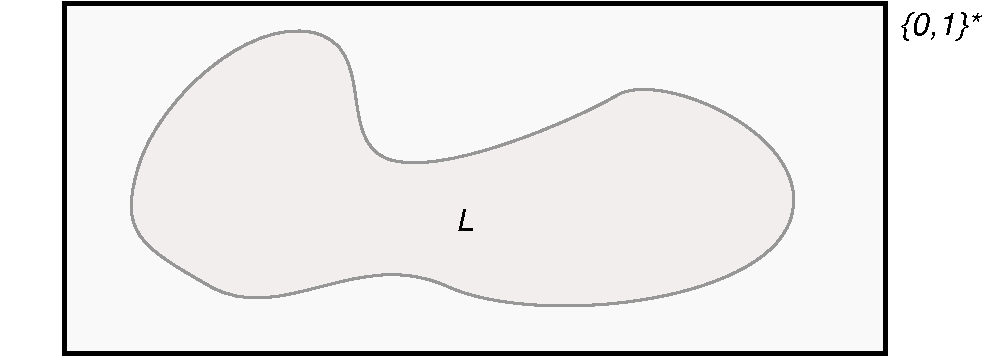
\includegraphics[width=0.7\textwidth]{sprog.pdf}
  \end{center}
  \caption{En delmængde (sprog) $L \subseteq \{0, 1\}^\ast$}
  \label{fig:sprog}
\end{figure}

Lad os nu betragte en Monte Carlo algoritme $A$ (one-sided error), så:
\begin{align*}
  x &\in L \rightarrow A(x) = 1 \text{ med sandsynlighed $\geq 1/2$}\\
  x &\notin L \rightarrow A(x) = 0 \text{ med sandsynlighed $1$}
\end{align*}

Antag at algoritme $A$ bruger $\lg n$ tilfældige bits repræsenteret som et tal $r \in \{0, ..., n-1 \}$ hvor $n$ er et primtal. I følgende bruger vi notationen $A(x, r)$ for at beskrive outputtet af $A$ på input $x$, hvor $A$ vælger den tilfældige bitstreng $r$. Og lad os i fejlsandsynlighederne antage, at vores konkrete $x \in L$ så det korrekte svar er 1.

\subsection{Algoritme 1 - $t \lg n$ random bits}
Vælg $t$ tal $r_0, \dots, r_{t-1} \in \{0, \dots, n-1\}$ uafhængigt og uniformt tilfældigt.\\
Beregn $A(x, r_0), \dots, A(x, r_{t-1})$. Hvis vi en enkelt gang ser tallet 1 er det bevis på $x \in L$, ellers hvis vi \emph{alle} gange får 0 vælger vi det som output.\\

Så vil fejlsandsynligheden være $< \pfrac{1}{2}^t = 1/2^t$.\\

Problemet ved denne tilgang er, at vi skal vælge $t \lg n$ random bits. Hvis vi f.eks. vælger $t = 2$ skal vi bruge $2 \ln n$ random bits for en fejlsandsynlighed $< 1/4$.

\subsection{Algoritme 2 - $2 \lg n$ random bits}
Vælg $a, b \in \curly{0, \dots, n-1}$ uafhængigt og uniformt tilfældigt.\\

Da vi antager $n$ er et primtal, så kan man vise at, for $X_i = (a * i + b) \bmod n$ vil $X_i$ og $X_j$ hvor $i \neq j$ være uniformt distribueret i $0, \dots, n-1$ og parvist uafhængige (kan blot antages, skal ikke bevises).\\

Med den info, lad $r_i = (a * i + b) \mod n$ for $i = 0, \dots, t-1$.\\
Igen beregner vi $A(x, r_0), \dots, A(x, r_{t-1})$ og vælger 1 såfremt den optræder bare én gang, ellers 0.\\

Nu bruger vi kun $2 \lg n$ random bits.

\subsection{Sandsynlighed for at algoritme 2 fejler}
Vi skal ligesom i randomized selection bruge, at givet parvis uafhængige stokastiske variable $Y_1, \dots, Y_m$ hvor vi lader $Y = \sum_{i=1}^m Y_i$, da er
\begin{align}
  {\sigma_Y}^2 = \sum_{i=1}^m {\sigma_{Y_i}}^2 \label{eq:parvis-uaf}
\end{align}\vspace{2em}

For $i = 0, \dots, t-1$ lader vi $Y_i = A(x, r_i)$. Lad nu $Y = \sum_{i=1}^{t-1} Y_i$.

Da kan vi beregne den forventede værdi:
\begin{align}
  \mu_Y = \sum_{i=0}^{t-1} \mu_{Y_i} = \sum_{i=0}^{t-1} p = tp \geq \frac{1}{2} \label{eq:mu-y-ulighed}
\end{align}
Idet vi lader symbolet $p = \P{Y_i = 1} \geq \frac{1}{2}$.\\

Derudover har vi jf. \cref{eq:parvis-uaf}, at hvis vi bruger samme logik som i \cref{eq:faa-paren} og \cref{eq:paren-to-max}, så får vi:
\begin{align*}
  {\sigma_Y}^2
  = \sum_{i=0}^{t-1} {\sigma_{Y_i}}^2
  = \sum_{i=0}^{t-1} p(1-p)
  \leq \frac{t}{4} \Longrightarrow \sigma_Y
  = \frac{\sqrt{t}}{2}
\end{align*}

Da kan vi beregne sandsynligheden for at algoritme 2 fejler til:
\begin{align}
  \P{\text{Algoritme 2 fejler}} &= \P{Y = 0} \label{eq:p-y-lig-0} \\
  &\leq \P{| Y - \mu_Y| \geq \frac{t}{2}} \label{eq:traak-middelvaardi} \\
  &= \P{|Y - \mu_Y| \geq \sqrt{t} \frac{\sqrt{t}}{2}} \nonumber \\
  &\leq \frac{1}{(\sqrt{t})^2} \label{eq:benyt-cheby}\\
  &\leq \frac{1}{t} \nonumber
\end{align}

I \cref{eq:p-y-lig-0} bruger vi, at algoritmen fejler (givet vores antagelse at svaret \emph{er} 1) når vi får 0 i alle vores trials.\\
I \cref{eq:traak-middelvaardi} indsætter vi ulighed \cref{eq:mu-y-ulighed} for $\mu_Y$. Grunden til vi får '$\leq$'-tegnet i denne ligning er pga. vi tager den absolutte værdi, hvorved der kommer ''to muligheder'' for at det udtryk kan være større end brøken, hvilket der ikke gjorde i \cref{eq:mu-y-ulighed}.\\
I \cref{eq:benyt-cheby} benytter vi Chebyshev's ulighed.\\

Hermed har vi altså bestemt, at vi kan få en relativt lav sandsynlighed for fejl selvom vi kun bruger $2 \lg n$ random bits.
